%%%%%%%%%%%%%%%%%%%%%%%%%%%%%%%%%%%%%%%%%%%%%%%%%%%%%%%%%%%%%%%%%%%%%%%%%%%%%%%%%%%%%
% PACOTES                                                                           %
%%%%%%%%%%%%%%%%%%%%%%%%%%%%%%%%%%%%%%%%%%%%%%%%%%%%%%%%%%%%%%%%%%%%%%%%%%%%%%%%%%%%%
\documentclass[a4paper,12pt]{article}

%-----------------------------------------------------------------------------------%
% LAYOUT DA PÁGINA                                                                  %
%-----------------------------------------------------------------------------------%
\usepackage[top=3cm, bottom=3cm, left=3cm, right=3cm]{geometry}
%\usepackage{fancyhdr} % Permite controlar como são exibidos os cabeçalhos

%-----------------------------------------------------------------------------------%
% FORMATAÇÃO DO TEXTO                                                               %
%-----------------------------------------------------------------------------------%
%\usepackage{setspace} % Permite definir o espaçamento entre linhas

%-----------------------------------------------------------------------------------%
% PACOTES DE IMAGENS                                                                %
%-----------------------------------------------------------------------------------%
\usepackage[pdftex]{graphicx}
\pdfsuppresswarningpagegroup=1 % A warning issued when several PDF images are
% imported in the same page. Mostly harmless, can be almost always supressed.
%\usepackage[pstarrows]{pict2e} % Amplia as funcionalidades do ambiente picture
\usepackage{tikz}
\usetikzlibrary{shapes, arrows, arrows.meta}

%-----------------------------------------------------------------------------------%
% PACOTES DE TABELAS                                                                %
%-----------------------------------------------------------------------------------%
\usepackage{array} % Facilita a formatação de tabelas
%\usepackage{multirow} % Permite criar células que ocupam várias linhas em uma tabela
\usepackage{longtable} % Permite criar tabelas que quebram de página

%-----------------------------------------------------------------------------------%
% PACOTES MATEMÁTICOS DE BASE                                                       %
%-----------------------------------------------------------------------------------%
\usepackage{amsfonts,amstext,amscd,bezier,amsthm,amssymb}
\usepackage[centertags]{amsmath}

%-----------------------------------------------------------------------------------%
% PACOTES DE SÍMBOLOS MATEMÁTICOS                                                   %
%-----------------------------------------------------------------------------------%
\usepackage{mathtools} % Símbolos matemáticos extras. (ex.: \xrightharpoon)
%\usepackage[integrals]{wasysym} % Muda o estilo das integrais, além de outros
%                                 símbolos extras
%\usepackage[nice]{nicefrac} % Permite o uso de frações "melhores". Usar \nicefrac{}{}

%-----------------------------------------------------------------------------------%
% PACOTES DE FONTES MATEMÁTICAS                                                     %
%-----------------------------------------------------------------------------------%
%\usepackage{mathbbol} % Quase todos os símbolos com \mathbb
%\usepackage{bbm} % Extensão dos símbolos de \mathbb. Usar comando \mathbbm
%\usepackage{calrsfs} % Muda o estilo de \mathcal
%\usepackage[mathcal]{euscript} % Muda o estilo de \mathcal

%-----------------------------------------------------------------------------------%
% PACOTES DE CODIFICAÇÃO DE FONTES                                                  %
%-----------------------------------------------------------------------------------%
\usepackage[utf8]{inputenc} % Permite o uso de caracteres ISO 8859-1, incluindo os
%                               caracteres acentuados diretamente.
\usepackage[T1]{fontenc} % Uso de fontes T1, necessário para tratar caracteres
%                          acentuados como um único bloco.

%-----------------------------------------------------------------------------------%
% PACOTES DE LÍNGUAS                                                                %
%-----------------------------------------------------------------------------------%
\usepackage[french]{babel} % Seleciona a língua do documento, definindo nomes de
%                              seções, nome do índice, da bibliografia, etc. Em caso
%                              de documento com mais de uma língua, a padrão é a
%                              última.
\NoAutoSpaceBeforeFDP % Utilizar em francês se quiser evitar espaços antes de :

%-----------------------------------------------------------------------------------%
% PACOTES DE BIBLIOGRAFIA                                                           %
%-----------------------------------------------------------------------------------%
%\usepackage{babelbib} % Permite definir a língua das entradas da bibliografia. Usar
%                       [fixlanguage] para uma mesma língua para todas as entradas e
%                       \selectbiblanguage{} para definir a língua. Um estilo compa-
%                       tível com babelbib deve ser usado (ex: babplain)
\usepackage{cite} % Organiza os elementos citados dentro de um mesmo \cite.

%-----------------------------------------------------------------------------------%
% PACOTES DE FONTES                                                                 %
%-----------------------------------------------------------------------------------%
% Computer Modern (fonte padrão)                                                    %
% - - - - - - - - - - - - - - - - - - - - - - - - - - - - - - - - - - - - - - - - - %
%\usepackage{ae} % A usar com a fonte padrão do LaTeX quando forem gerados PDFs, para
%                 corrigir erros de visualização

% Computer Modern Bright (sans serif)                                               %
% - - - - - - - - - - - - - - - - - - - - - - - - - - - - - - - - - - - - - - - - - %
%\usepackage{cmbright}

% Times New Roman                                                                   %
% - - - - - - - - - - - - - - - - - - - - - - - - - - - - - - - - - - - - - - - - - %
%\usepackage{mathptmx} % Muda texto e modo matemático
%\usepackage{times} % Apenas texto, não muda modo matemático

% Arial                                                                             %
% - - - - - - - - - - - - - - - - - - - - - - - - - - - - - - - - - - - - - - - - - %
%\usepackage[scaled]{uarial} % Arial como fonte sans serif padrão

% Palatino                                                                          %
% - - - - - - - - - - - - - - - - - - - - - - - - - - - - - - - - - - - - - - - - - %
%\usepackage{mathpazo} % Muda texto e modo matemático
%\usepackage{palatino} % Apenas texto, não muda modo matemático

% Concrete                                                                          %
% - - - - - - - - - - - - - - - - - - - - - - - - - - - - - - - - - - - - - - - - - %
%\usepackage{ccfonts} % Texto: Concrete; Matemático: Concrete Math
%\usepackage{ccfonts, eulervm} % Texto: Concrete; Matemático: Euler

% Iwona                                                                             %
% - - - - - - - - - - - - - - - - - - - - - - - - - - - - - - - - - - - - - - - - - %
%\usepackage[math]{iwona} % Texto e modo matemático: Iwona

% Kurier                                                                            %
% - - - - - - - - - - - - - - - - - - - - - - - - - - - - - - - - - - - - - - - - - %
%\usepackage[math]{kurier} % Texto e modo matemático: Kurier

% Antykwa Póltawskiego                                                              %
% - - - - - - - - - - - - - - - - - - - - - - - - - - - - - - - - - - - - - - - - - %
%\usepackage{antpolt} % Texto: Antykwa Póltawskiego; Matemático: nenhum
                     % Usar fontenc = QX ou OT4

% Utopia                                                                            %
% - - - - - - - - - - - - - - - - - - - - - - - - - - - - - - - - - - - - - - - - - %                     
%\usepackage{fourier} % Texto: Utopia; Matemático: Fourier

% KP Serif                                                                          %
% - - - - - - - - - - - - - - - - - - - - - - - - - - - - - - - - - - - - - - - - - %
\usepackage{kpfonts}

%-----------------------------------------------------------------------------------%
% CORES                                                                             %
%-----------------------------------------------------------------------------------%
\usepackage{color}
\definecolor{darkgreen}{rgb}{0,0.5,0}
\definecolor{darkmagenta}{rgb}{0.5,0,0.5}
\definecolor{darkgray}{rgb}{0.5,0.5,0.5}
\definecolor{darkblue}{rgb}{0.2,0.2,0.4}
\definecolor{darkred}{rgb}{0.6,0.15,0.15}
\definecolor{gray}{rgb}{0.65,0.65,0.65}
\definecolor{lightgray}{rgb}{0.8,0.8,0.8}
\definecolor{lightblue}{rgb}{0.5,0.5,1}
\definecolor{lightgreen}{rgb}{0.5,1,0.5}
\definecolor{deadred}{rgb}{0.7, 0.2, 0.2}
\definecolor{deadblue}{rgb}{0.2, 0.2, 0.7}

%-----------------------------------------------------------------------------------%
% PACOTES DIVERSOS                                                                  %
%-----------------------------------------------------------------------------------%
\usepackage{icomma} % Permite uso de vírgula como separador decimal
\usepackage{url} % Pacote para não ter problemas com URLs. Usar \url{}
%\usepackage{randtext} % Troca a ordem de letras de uma frase (útil com e-mails em
                      % PDFs a serem publicados on-line.
\usepackage[hidelinks]{hyperref}
%\usepackage{showkeys} % Para mostrar o nome dos labels
\usepackage{enumitem} % Facilita o uso de listas, inclusive referências a itens de
                      % listas.
%\usepackage[absolute]{textpos} % Posição absoluta de texto na página
%\usepackage{pdfpages} % Permite incluir documentos em PDF no arquivo
%\usepackage{refcheck} % Verifica as referências procurando por
%                      % labels não usados ou equações numeradas sem labels.
%                      % Verificar o arquivo .log e procurar por RefCheck.
\usepackage[french, onelanguage]{algorithm2e}

%%%%%%%%%%%%%%%%%%%%%%%%%%%%%%%%%%%%%%%%%%%%%%%%%%%%%%%%%%%%%%%%%%%%%%%%%%%%%%%%%%%%%
% CONFIGURAÇÕES                                                                     %
%%%%%%%%%%%%%%%%%%%%%%%%%%%%%%%%%%%%%%%%%%%%%%%%%%%%%%%%%%%%%%%%%%%%%%%%%%%%%%%%%%%%%

%-----------------------------------------------------------------------------------%
% FORMATAÇÃO DO TEXTO                                                               %
%-----------------------------------------------------------------------------------%
%\onehalfspacing % Espaçamento 1 1/2 (definido no pacote setspace)

%-----------------------------------------------------------------------------------%
% DEFINIÇÃO DE AMBIENTES MATEMÁTICOS                                                %
%-----------------------------------------------------------------------------------%
%\theoremstyle{plain}
%\newtheorem{theo}{Teorema}[section]
%\newtheorem{lemm}[theo]{Lema}
%\newtheorem{coro}[theo]{Corolário}
%\newtheorem{prop}[theo]{Proposição}
%\theoremstyle{definition}
%\newtheorem{defi}[theo]{Definição}
%\newtheorem{remq}[theo]{Observação}
%%\newtheorem{expl}[theo]{Exemplo}
%\newenvironment{expl}%
%  {\refstepcounter{theo}%
%    \begin{list}{}{%
%    \setlength{\topsep}{0pt}%
%    \setlength{\leftmargin}{\parindent}%
%    \setlength{\rightmargin}{0pt}%
%    \setlength{\listparindent}{\parindent}%
%    \setlength{\itemindent}{0pt}%
%    \setlength{\parsep}{\parskip}}%
%    \item[]{\bf Exemplo \thetheo. }}%
%  {\hspace*{\fill} $\square$ \end{list} \medskip}
%\newenvironment{solu}%
%  {\noindent {\bf Solução. }\small}%
%  {\hspace*{\fill} $\square$ \normalsize \medskip}
%\newenvironment{dems}[1][Demonstração]%
%  {\begin{list}{}{%
%    \setlength{\topsep}{0pt}%
%    \setlength{\leftmargin}{\parindent}%
%    \setlength{\rightmargin}{0pt}%
%    \setlength{\listparindent}{\parindent}%
%    \setlength{\itemindent}{0pt}%
%    \setlength{\parsep}{\parskip}}%
%    \item[]{\bf #1. }}%
%  {\hspace*{\fill} $\blacksquare$ \end{list} \medskip}


%-----------------------------------------------------------------------------------%
% DEFINIÇÃO DE COMANDOS MATEMÁTICOS                                                 %
%-----------------------------------------------------------------------------------%
%\newcommand*\diff{\mathop{}\!\mathrm{d}}

%\newcommand{\norm}[1]{\left\lVert #1\right\lVert} % Norma
%\newcommand{\abs}[1]{\left\lvert #1\right \rvert} % Valor absoluto
%\newcommand{\floor}[1]{\left\lfloor #1 \right\rfloor} % Arredondar para baixo
%\newcommand{\ceil}[1]{\left\lceil #1 \right\rceil} % Arredondar para cima
\DeclarePairedDelimiter{\ceil}{\lceil}{\rceil}
\DeclareMathOperator*{\argmax}{argmax}

%-----------------------------------------------------------------------------------%
% NUMERAÇÃO DE ELEMENTOS                                                            %
%-----------------------------------------------------------------------------------%
%\numberwithin{table}{section}
%\numberwithin{table}{subsection}
%\numberwithin{figure}{section}
%\numberwithin{figure}{subsection}
%\numberwithin{equation}{section}
%\numberwithin{equation}{subsection}
%\numberwithin{theo}{chapter}
%\numberwithin{theo}{subsection}

% Maximal percentage of the page occupied by floats
\renewcommand\floatpagefraction{.9}
\renewcommand\topfraction{.9}
\renewcommand\bottomfraction{.9}
\renewcommand\textfraction{.1}
% Maximal number of floats per page
\setcounter{totalnumber}{50}
\setcounter{topnumber}{50}
\setcounter{bottomnumber}{50}

%%%%%%%%%%%%%%%%%%%%%%%%%%%%%%%%%%%%%%%%%%%%%%%%%%%%%%%%%%%%%%%%%%%%%%%%%%%%%%%%%%%%%
% ESTRUTURA DO DOCUMENTO                                                            %
%%%%%%%%%%%%%%%%%%%%%%%%%%%%%%%%%%%%%%%%%%%%%%%%%%%%%%%%%%%%%%%%%%%%%%%%%%%%%%%%%%%%%
\begin{document}

\pagestyle{plain}

\title{3I005 \\ Projet 3 : Analyse de séquences génomiques}
\author{Ariana Carnielli \\ Yasmine Ikhelif}
\date{}

\maketitle

\sloppy

\tableofcontents

\section{Introduction}

Les valeurs présentées dans ce document ont été calculées à l'aide des codes en Python dans le fichier \verb@projet.py@, qui contient l'implémentation des fonctions demandées, et dans le Jupyter Notebook \verb@Projet3.ipynb@, qui contient les appels de ces fonctions et l'affichage des résultats.

\section{Préliminaires : données et lecture des fichiers}

\subsubsection*{Question 1}

Quatre fichiers ont été données pour ce projet. Leurs noms et les nombres de séquences et de nucléotides dans chacun d'entre eux sont présentés dans le tableau ci-dessous.

\begin{center}
\begin{tabular}{l >{\centering} m{2.75cm} >{\centering} m{2.75cm}}
Nom du fichier & Nombre de séquences & Total de nucléotides \tabularnewline
\hline
\verb@regulatory_seq_PHO.fasta@ & 5 & 4000 \tabularnewline
\verb@regulatory_seqs_GAL.fasta@ & 7 & 5608 \tabularnewline
\verb@regulatory_seqs_MET.fasta@ & 9 & 7200 \tabularnewline
\verb@yeast_s_cerevisae_genomic_chr1-4.fna@ & 4 & 2515853 \tabularnewline
\end{tabular}
\end{center}

Les chromosomes de \emph{S.\ cerevisae} donnés dans le fichier \texttt{yeast\_\allowbreak{}s\_\allowbreak{}cerevisae\_\allowbreak{}genomic\_\allowbreak{}chr1-4\allowbreak{}.fna} contiennent ainsi 2515853 nucléotides.

\subsubsection*{Question 2}

L'application de la fonction \verb@nucleotide_frequency@ à la liste des nucléotides de \emph{S.\ cerevisae} donnés dans le fichier \texttt{yeast\_\allowbreak{}s\_\allowbreak{}cerevisae\_\allowbreak{}genomic\_\allowbreak{}chr1-4\allowbreak{}.fna} donne les fréquences présentées dans le tableau ci-dessous.

\begin{center}
\begin{tabular}{cc}
Nucléotide & Fréquence \tabularnewline
\hline
A & 0.29984 \tabularnewline
C & 0.20110 \tabularnewline
G & 0.20000 \tabularnewline
T & 0.29907 \tabularnewline
\end{tabular}
\end{center}

\subsubsection*{Questions 3 et 4}

Les fonctions \verb@logproba@ et \verb@logprobafast@ ont été codées dans \verb@projet.py@ et testées dans \verb@Projet3.ipynb@.

\section{Annotation des régions promoteurs}

\subsection{Description Empirique, préliminaires}

\subsubsection*{Question 1}

Les fonctions \verb@code@, \verb@inverse@ et \verb@comptage@ ont été codées dans \verb@projet.py@ et testées dans \verb@Projet3.ipynb@.

\subsubsection*{Question 2}

On fixe un mot $w = w_0 w_1 \dotsm w_{k-1}$ de longueur $k$ et on considère une séquence aléatoire de longueur $\ell$, $S_0 S_1 \dotsm S_{\ell - 1}$ avec $\ell \geq k$. On suppose que les variables aléatoires $S_0, \dotsc, S_{\ell-1}$ correspondant à chaque lettre sont indépendantes et identiquement distribuées (leur loi étant estimée par la fonction donnée \verb@nucleotide_frequency@). Soit $X_i$ la variable aléatoire Bernoulli qui vaut $1$ si et seulement si le mot $w$ apparait dans $S$ à la case $i$, c'est-à-dire $S_i = w_0$, $S_{i+1} = w_1$, $\dotsc$, $S_{i + k - 1} = w_{k-1}$. Remarquons que cela n'est possible que si $i + k - 1 \leq \ell - 1$, donc $i \leq \ell - k$. Comme les variables $S_j$ sont indépendantes, on a
\[
P(X_i = 1) = P(S_i = w_0) P(S_{i+1} = w_1) \dotsm P(S_{i+k-1} = w_{k-1}).
\]
De plus, comme les variables $S_j$ sont identiquement distribuées, $P(X_i = 1)$ ne dépend pas de $i$ (mais dépend de $w$). Notons $p = P(X_i = 1)$. Remarquons que $p$ n'est rien d'autre que l'exponentielle de la valeur rendue par la fonction \verb@logproba@ lorsque son argument \verb@liste_entiers@ vaut $w$ et son argument \verb@m@ contient la loi des $S_j$.

Soit $X$ la variable aléatoire donnant le nombre d'occurrences de $w$ dans $S$. On a alors
\[
X = \sum_{i=0}^{\ell - k} X_i.
\]
On remarque que, sauf dans le cas $k = 1$, les variables $X_i$ ne sont pas indépendantes, donc $X$ n'est pas forcément une variable aléatoire binomiale. Cependant, comme l'espérance est linéaire et $\mathbb E(X_i) = P(X_i = 1) = p$ car $X_i$ suit une loi de Bernoulli, on peut calculer l'espérance de $X$ par
\[
\mathbb E(X) = \sum_{i=0}^{\ell - k} \mathbb E(X_i) = \sum_{i=0}^{\ell - k} p = p (\ell - k + 1).
\]
Cette formule a été implémentée dans la fonction \verb@comptage_attendu@ codée dans le fichier \verb@projet.py@ et testée dans le fichier \verb@Projet3.ipynb@.

\subsubsection*{Question 3}

Les graphiques, obtenus dans le fichier \verb@Projet3.ipynb@, sont données dans la Figure \ref{FigNbOccurrences}. On y remarque qu'il y a un écart important entre les nombres d'occurrence attendus et observés, qui peut être vu par la distance entre les points tracés et la diagonale, représentée en gris sur les figures. Cet écart est d'autant plus important que la longueur du mot recherché est grand. Ainsi, le modèle utilisé jusqu'à présent, qui suppose que deux lettres à des positions différentes sont des variables aléatoires indépendantes, ne permet pas d'expliquer les observations des occurrences des mots. Certains mots sont beaucoup plus fréquents que d'autres et cela ne peut pas être expliqué simplement par les fréquences de leurs lettres.

\begin{figure}
\centering
\begin{tabular}{@{} c @{} c @{}}
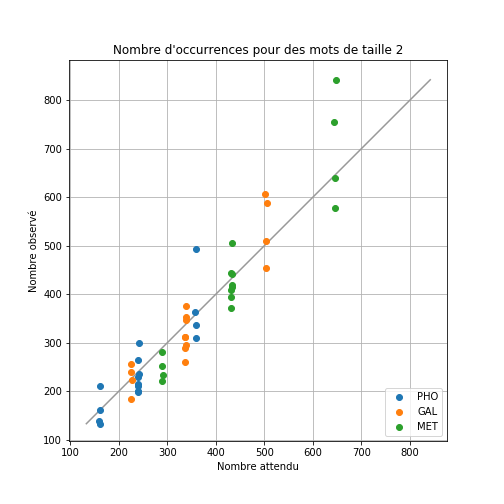
\includegraphics[width=0.5\textwidth]{Figures/graphe_occurrences_2.png} & 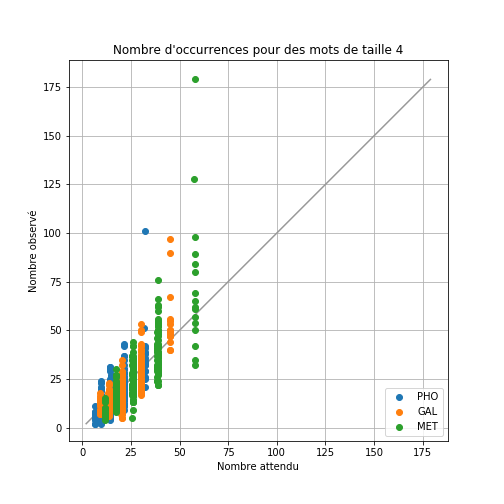
\includegraphics[width=0.5\textwidth]{Figures/graphe_occurrences_4.png} \tabularnewline
(a) & (b) \tabularnewline
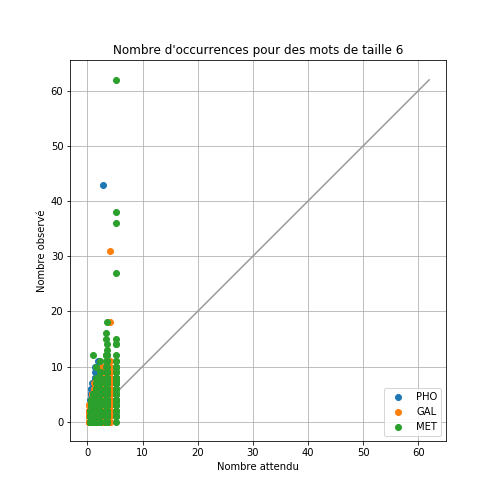
\includegraphics[width=0.5\textwidth]{Figures/graphe_occurrences_6.png} & 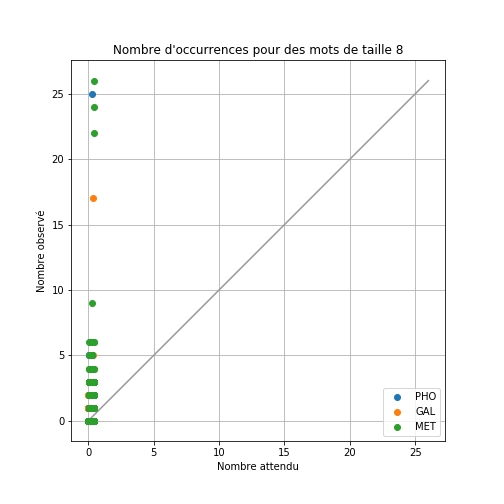
\includegraphics[width=0.5\textwidth]{Figures/graphe_occurrences_8.png} \tabularnewline
(c) & (d) \tabularnewline
\end{tabular}
\caption{Nombre d'occurrences attendu et observé pour (a) $k = 2$, (b) $k = 4$, (c) $k = 6$ et (d) $k = 8$.}
\label{FigNbOccurrences}
\end{figure}

\subsection{Simulation de séquences aléatoires}

\subsubsection*{Question 1}

La fonction \verb@simule_sequence@ a été codée dans \verb@projet.py@ et testée dans \verb@Projet3.ipynb@. Pour la création de la séquence, on suppose que les lettres à des positions différentes sont indépendantes.

\subsubsection*{Question 2}

On a simulé des séquences de grande longueur et tracé le graphique avec les nombres attendus et observées de chaque mot de longueurs $k$ données. Les résultats pour une séquence de taille 1000000 et $k = 6$ sont donnés dans la Figure \ref{FigOccurrencesSimul}. On y observe que les points sont assez proches de la diagonale, comme attendu, car le calcul du nombre d'occurrences attendu se base sur l'indépendance des lettres de la séquence, utilisée pour la création de la séquence aléatoire. Ces points sont d'autant plus proches de la diagonale que la taille de la séquence générée est grande mais leur variance, et donc leur dispersion autour de la diagonale, augmente rapidement avec $k$.

\begin{figure}
\centering
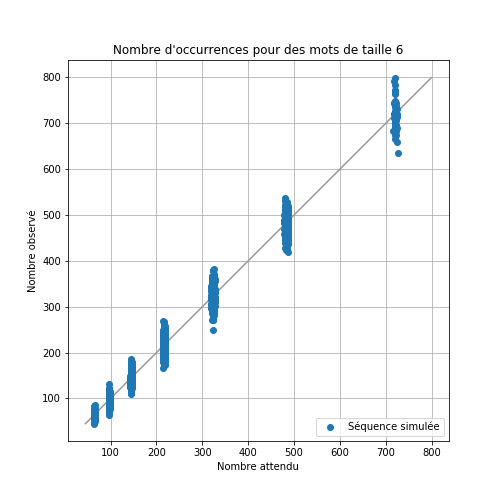
\includegraphics[width=0.6\textwidth]{Figures/graphe_occurrences_simul.png}
\caption{Nombre d'occurrences attendu et observé pour une séquence de taille 1000000 générée aléatoirement.}
\label{FigOccurrencesSimul}
\end{figure}

\subsubsection*{Question 3}

La fonction \verb@proba_empirique@ calculant la probabilité empirique d'un mot a été codée dans \verb@projet.py@ et testée dans \verb@Projet3.ipynb@. Elle prend en argument un mot, la taille \verb@lg@ de la séquence à simuler, les probabilités de chaque nucléotide et un nombre de simulations à faire et renvoie un dictionnaire tel que l'élément de clé \verb@i@ contient la probabilité estimée que ce mot apparaisse exactement \verb@i@ fois dans une séquence de taille \verb@lg@.

\subsubsection*{Question 4}

La Figure \ref{FigHistogrammes} donne les histogrammes avec les probabilités estimées du nombre d'occurrences des mots ATCTGC, ATATAT, TTTAAA et AAAAAA pour des suites de longueur 10000 en faisant 1000 simulations pour chaque mot. Le code pour créer ces figures est donné dans le fichier \verb@Projet3.ipynb@.

\begin{figure}
\centering
\begin{tabular}{@{} c @{} c @{}}
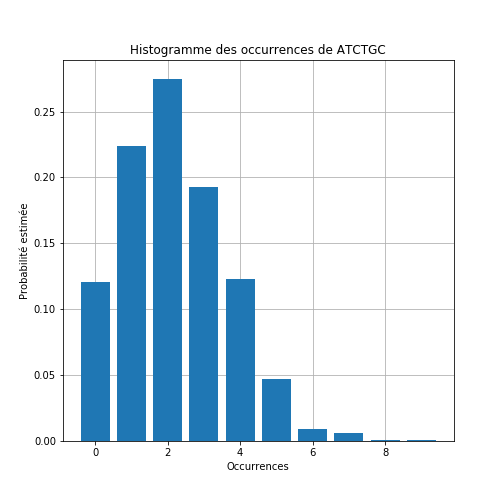
\includegraphics[width=0.5\textwidth]{Figures/histogramme_ATCTGC.png} & 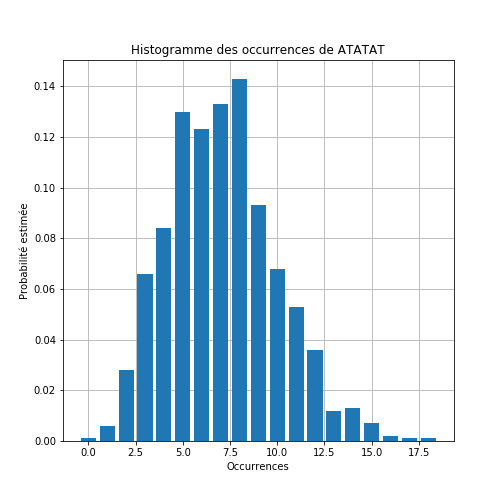
\includegraphics[width=0.5\textwidth]{Figures/histogramme_ATATAT.png} \tabularnewline
(a) & (b) \tabularnewline
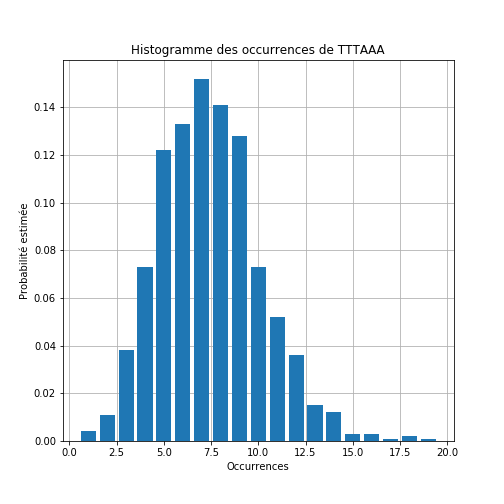
\includegraphics[width=0.5\textwidth]{Figures/histogramme_TTTAAA.png} & 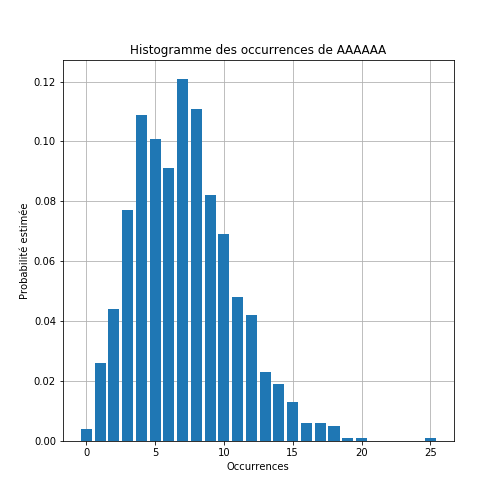
\includegraphics[width=0.5\textwidth]{Figures/histogramme_AAAAAA.png} \tabularnewline
(c) & (d) \tabularnewline
\end{tabular}
\caption{Histogrammes avec les probabilités estimées du nombre d'occurrences des mots (a) ATCTGC, (b) ATATAT, (c) TTTAAA et (d) AAAAAA.}
\label{FigHistogrammes}
\end{figure}

On observe dans la figure que les probabilités d'occurrence dépendent du mot en question. Cela dépend des lettres qui composent ce mot, car A et T sont plus fréquentes que C et G, ce qui explique la différence de la Figure \ref{FigHistogrammes}(a) avec les trois autres, mais les probabilités dépendent aussi du mot en soi. En effet, certains mots peuvent se chevaucher plus facilement, en on espère ainsi avoir des nombres d'occurrence plus grands de ces mots. Par exemple, en supposant les lettres A et T comme équiprobables, les séquences à 12 lettres ATATATATATAT, TTTAAATTTAAA et AAAAAAAAAAAA ont toutes la même probabilité d'apparaitre, mais la première donne lieu à 4 occurrences du mot ATATAT, la deuxième donne lieu à 2 occurrences du mot TTTAAA et la troisième donne lieu à 7 occurrences du mot AAAAAA, cette dernière étant la séquence qui s'auto-chevauche le plus facilement. En particulier, dans une séquence de longueur $\ell$ avec $\ell$ un multiple de 6, le nombre maximal d'occurrences du mot AAAAAA est $\ell - 6 + 1$, le nombre maximal d'occurrences de ATATAT est $\frac{\ell}{2} - 2$ et le nombre maximal d'occurrences de TTTAAA est $\frac{\ell}{6}$, ce qui indique déjà que les lois de probabilité du nombre d'occurrences de ces mots sont différents car leurs supports sont différents.

\subsubsection*{Question 5}

Fixons un mot $w$ et deux entiers $n$ et $\ell$. Soit $N$ la variable aléatoire représentant le nombre d'occurrences de $w$ dans des séquences aléatoires de longueur $\ell$. Pour estimer $p = P(N = n)$, on peut considérer que $p$ est le paramètre d'une variable aléatoire de loi Bernoulli qui vaut $1$ si $N = n$ et $0$ sinon. On peut alors utiliser l'intervalle de confiance pour une loi de Bernoulli, donné par
\[
I = \left[\hat p - t_\alpha \sqrt{\frac{\hat p (1 - \hat p)}{N}}, \hat p + t_\alpha \sqrt{\frac{\hat p (1 - \hat p)}{N}}\right]
\]
où $\hat p$ est la valeur estimée de $p$ et $t_\alpha$ est calculé à partir du niveau de confiance $\alpha$, avec $t_\alpha \approx 1,96$ si $\alpha = 0,05$. La Figure \ref{FigHistogrammeErrorBar} représente l'histogramme du nombre d'occurrences du mot ATATAT avec des barres représentant les intervalles de confiance de chaque probabilité calculés à l'aide de la formule ci-dessus et $\alpha = 0,05$. Les histogrammes avec les intervalles de confiance pour les autres mots sont donnés dans le fichier \verb@Projet3.ipynb@.

\begin{figure}
\centering
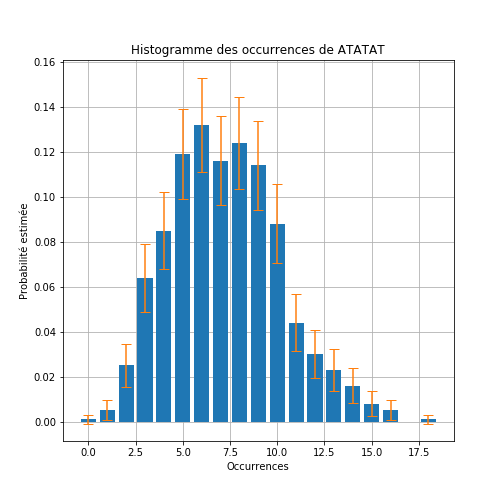
\includegraphics[width=0.6\textwidth]{Figures/histogramme_ATATAT_errorbar.png}
\caption{Histogrammes avec les probabilités estimées et les intervalles de confiance pour le nombre d'occurrences du mot ATATAT.}
\label{FigHistogrammeErrorBar}
\end{figure}


\end{document}
